\chapter{Analisi Numerica}
\section{Introduzione}
In questo capitolo verranno presentate alcune tecniche per la risoluzione dei
sistemi lineari e il concetto di \textbf{numero di condizionamento}.

Lo sviluppo di un algoritmo di risoluzione di sistemi lineari deve considerare
tre fattori:
\begin{enumerate}
    \item \textbf{Memoria}: l'algoritmo deve richiedere un quantitativo ridotto
          di memoria.
    \item \textbf{Velocità}: l'algoritmo deve essere molto veloce.
    \item \textbf{Precisione}: vogliamo ottenere una soluzione più vicina possibile
          a quella reale.
\end{enumerate}
\subsection{Gestione di Matrici e Vettori}
A livello di programmazione, i vettori possono essere salvati utilizzando
aree congiunte di memoria (array). Mentre, per quanto riguarda le matrici, si
possono salvare in array secondo diverse filosofie:
\begin{itemize}
    \item \textbf{Row Major}: si salvano le righe una dopo l'altra.
          \begin{figure}[!ht]
              \centering
              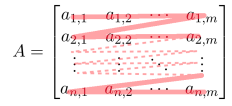
\includegraphics[width=0.25\textwidth]{./img/AnalisiNumerica/RowMajor.png}
              \caption{Esempio di salvataggio di una matrice in Row Major}
          \end{figure}
    \item \textbf{Column Major}: si salvano le colonne una dopo l'altra.
          \begin{figure}[!ht]
              \centering
              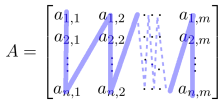
\includegraphics[width=0.25\textwidth]{./img/AnalisiNumerica/ColumnMajor.png}
              \caption{Esempio di salvataggio di una matrice in Column Major}
          \end{figure}
\end{itemize}

Per salvare una matrice \textbf{sparsa} viene sempre salvata come collezione di
tuple $\langle i, \, j,\, val\rangle$. Con questa rappresentazione, anche nota
come \textbf{formato sparso}, ogni qualvolta si effettua un'operazione tra matrici
sparse si trasformano in matrici normali e si applica l'operazione.
\subsection{Gestione Errori}
L'algoritmo creato deve essere valutato in base a quanto è vicino il risultato
restituito rispetto a quello corretto. Questo deve essere fatto in quanto
i risultati sono spesso forniti come numeri floating point e quindi soggetti
a errori di approssimazione.

\begin{definizione}[\textbf{Errore assoluto}]
    Sia $\stackrel{\sim}{\textbf{x}}$ la soluzione approssimata di un sistema
    lineare $A\textbf{x} = \textbf{b}$ e sia $x$ la soluzione corretta, allora
    l'\textbf{errore assoluto} è definito come:
    \begin{equation}
        \epsilon = \|\stackrel{\sim}{\textbf{x}} - \textbf{x}\|
    \end{equation}
    dove $\|\cdot\|$ è una qualsiasi norma fra due vettori.
\end{definizione}
\begin{definizione}[\textbf{Errore relativo}]
    Sia $\stackrel{\sim}{\textbf{x}}$ la soluzione approssimata di un sistema
    lineare $A\textbf{x} = \textbf{b}$ e sia $x$ la soluzione corretta, allora
    l'\textbf{errore relativo} è definito come:
    \begin{equation}
        \epsilon = \frac{\|\stackrel{\sim}{\textbf{x}} - \textbf{x}\|}{\|\textbf{x}\|}
    \end{equation}
    dove $\|\cdot\|$ è una qualsiasi norma fra due vettori.
\end{definizione}
\begin{teorema}\label{teo:NormeEquivalenti}
    Il comportamento delle norme di vettori in $\mathbb{R}^n$ è equivalente. ossia
    preso un vettore $x\in \mathbb{R}^n$, $\exists c_1,c_2\in \mathbb{R}$ tali che:
    \begin{equation}
        c_1\|x\|_p < \|x\|_q < c_2\|x\|_p
    \end{equation}
\end{teorema}
Il teorema \ref{teo:NormeEquivalenti} ci dice che le norme a meno di alcuni
fattori moltiplicativi restituiscono gli stessi risultati.
\subsection{Velocità}
Come precedentemente detto, un aspetto importante è la velocità dell'algoritmo.
Per calcolare questo parametro dobbiamo contare il numero di operazioni che
effettuiamo, nello specifico si andrà ad utilizzare la complessità asintotica.

Analizziamo ora le velocità delle diverse operazioni:
\begin{itemize}
    \item \textbf{Prodotto Scalare}: sia $(x,y) = \sum_{i=1}^n x_iy_i$ corrisponde
          ad effettuare $n$ prodotti e $n-1$ somme, quindi si ha $n + n - 1 = 2
              n -1 \in \mathcal{O}(n)$
    \item \textbf{Norma di un vettore}: sia $\|x\| = \sqrt{\sum_{i=1}^n x_i^2}$
          corrisponde ad effettuare $n$ prodotti e $n-1$ somme, quindi si ha
          $n + n - 1 = 2n -1 \in \mathcal{O}(n)$
    \item \textbf{Prodotto Matrice-Vettore}: siano $A\in \mathbb{R}^{r\times c}$
          e $v\in \mathbb{R}^c$ allora $Av\in \mathcal{O} (rc) = \mathcal{O}(n^2)$
    \item \textbf{prodotto Matrice-Matrice}: siano $A,B\in \mathbb{R}^{n\times n}$
          allora $AB\in \mathcal{O} (n \cdot n \cdot n) = \mathcal{O} (n^3)$
    \item \textbf{Determinate}: sia $A\in \mathbb{R}^{n\times n}$ allora
          $det(A) \in \mathcal{O}(n!)$.
\end{itemize}
\section{Numero di Condizionamento}
Sappiamo che presa una matrice $A \in \mathbb{R}^{n \times n}$ e un vettore $b
    \in \mathbb{R}^n$ diverso dal vettore nullo, il sistema lineare $A \textbf{x} =
    \textbf{b}$ ammette soluzione se e soltanto se $det(A) \neq 0$.

Purtroppo quando si risolvono i sistemi lineari al calcolatore subentrano una
serie di altri fattori che influenzano il modo in cui si risolve il sistema e,
di conseguenza, la soluzione stessa. Questi fattori sono dovuti essenzialmente
alla rappresentazione dei numeri e agli errori di arrotondamento nelle operazioni.

Oltre a ciò, analizzando le velocità delle operazioni, si può notare che il
calcolo del determinante è molto complesso, quindi non è possibile utilizzarlo
per capire se un sistema è complesso da risolvere.

Per ovviare a questo problema, si introduce il concetto di \textbf{numero di
    condizionamento} calcolato su una matrice. Se tale valore è alto allora il
sistema è complesso da risolvere.
\begin{definizione}[\textbf{Numero di Condizionamento}]
    Presa una matrice $A \in \mathbb{R}^{n \times n}$, il \textbf{numero di
        condizionamento} è definito come:
    \begin{equation}
        cond(A) = \|\lambda_{max}\| \cdot \|\lambda_{min}\|
    \end{equation}
    dove $\lambda_{max}$ e $\lambda_{min}$ sono rispettivamente il massimo e il
    minimo autovalore della matrice $A$ in modulo.
\end{definizione}
Per definizione il numero di condizionamento è una quantità maggiore di $1$.
Vedremo che più questa quantità è vicino a $1$ più il sistema sarà facile da
risolvere numericamente, ossia risente meno dell'algebra di macchina. Di contro
più grande è questa quantità più il sistema sarà risolto “male”.
\begin{esempio}[Numero di Condizionamento di una Matrice di Hillbert]
    Prendiamo una matrice $H \in \mathbb{R}^{n \times n}$ definita nel seguente modo:
    \begin{equation*}
        H_{ij}=\frac{1}{1+i+j}
    \end{equation*}
    Questa matrice è nota con il nome di matrice di Hillbert ed è il classico
    esempio di matrice mal condizionata. 
\end{esempio}